\documentclass{article}
\usepackage{bm}
\usepackage{amssymb}
\usepackage{tikz}
\usetikzlibrary{positioning}

\title{Basic MLP with manually-derived Backprop}
\author{Teo Asinari}
\date{\today}

\begin{document}
\maketitle

\section{Introduction}
\paragraph{Goal:} To design, train and use a simple 3-layer MLP for binary classification
of size-2 vectors.
\paragraph{Design:} of the form \[[(layer\_size, Activation)...]\]: [(2, ReLU), (2, ReLU), (1, Sigmoid)]
\subsection{Diagrams}
\subsubsection{Vectorized Diagram (Equiv to Roger Grosse' 'Computational Graph')}
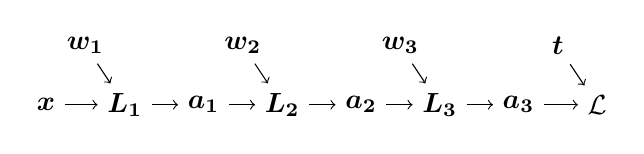
\begin{tikzpicture}[]
    \node (input) at (1,1) {$\bm{x}$};
    \node (weight1) at (1.5,1.75) {$\bm{w_1}$};
    \node (inputLayer) at (2,1) {$\bm{L_1}$};
    \node (activation1) at (3,1) {$\bm{a_1}$};
    \node (hiddenLayer) at (4,1) {$\bm{L_2}$};
    \node (weight2) at (3.5,1.75) {$\bm{w_2}$};
    \node (activation2) at (5,1) {$\bm{a_2}$};
    \node (outputLayer) at (6,1) {$\bm{L_3}$};
    \node (weight3) at (5.5,1.75) {$\bm{w_3}$};
    \node (activation3) at (7,1) {$\bm{a_3}$};
    \node (target) at (7.5,1.75) {$\bm{t}$};
    \node (loss) at (8,1) {$\mathcal{L}$};


\draw[->] (input) -- (inputLayer);
\draw[->] (weight1) -- (inputLayer);
\draw[->] (inputLayer) -- (activation1);
\draw[->] (activation1) -- (hiddenLayer);
\draw[->] (weight2) -- (hiddenLayer);
\draw[->] (hiddenLayer) -- (activation2);
\draw[->] (activation2) -- (outputLayer);
\draw[->] (weight3) -- (outputLayer);
\draw[->] (outputLayer) -- (activation3);
\draw[->] (target) -- (loss);
\draw[->] (activation3) -- (loss);

\end{tikzpicture}
\subsubsection{Expanded Diagram (Equiv. to Roger Grosse' 'Network Architecture')}
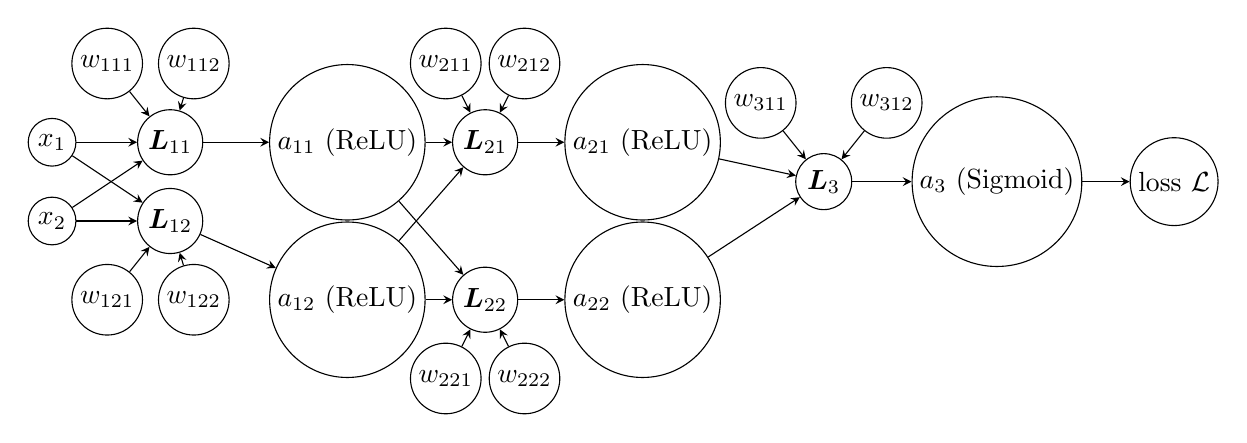
\begin{tikzpicture}[%
    activation/.style={%
        draw,
        circle,
        inner sep=2pt,
        minimum size=0.5cm,
        node distance=0.5cm
    },
    input/.style={%
        draw,
        circle,
        inner sep=2pt,
        minimum size=0.5cm,
        node distance=0.5cm
    },
    weight/.style={%
        draw,
        circle,
        inner sep=2pt,
        minimum size=0.5cm,
        node distance=0.5cm
    },
    inputLayer/.style={%
        draw,
        circle,
        inner sep=2pt,
        minimum size=0.5cm,
        node distance=0.5cm
    },
    hidden/.style={%
        draw,
        circle,
        inner sep=2pt,
        minimum size=0.5cm,
        node distance=0.5cm
    },
    output/.style={%
        draw,
        circle,
        inner sep=2pt,
        minimum size=0.5cm,
        node distance=0.5cm
    },
    >=stealth
]

% Inputs
    \node[input] (input1) at (1,1) {$x_1$};
    \node[input] (input2) at (1,0) {$x_2$};

% Input layer 1 (L_1)
    \node[inputLayer] (inputLayer1) at (2.5,1) {$\bm{L}_{11}$};
    \node[inputLayer] (inputLayer2) at (2.5, 0) {$\bm{L}_{12}$};
    \node[weight] (weight111) at (1.7, 2) {$w_{111}$};
    \node[weight] (weight112) at (2.8, 2) {$w_{112}$};
    \node[weight] (weight121) at (1.7, -1) {$w_{121}$};
    \node[weight] (weight122) at (2.8, -1) {$w_{122}$};

% Input Layer Activation
    \node[activation] (activation11) at (4.75, 1) {$a_{11}$ (ReLU)};
    \node[activation] (activation12) at (4.75, -1) {$a_{12}$ (ReLU)};

% Hidden layer 2 (L_2)
    \node[hidden] (hidden1) at (6.5, 1) {$\bm{L}_{21}$};
    \node[hidden] (hidden2) at (6.5, -1) {$\bm{L}_{22}$};
    \node[weight] (weight211) at (6, 2) {$w_{211}$};
    \node[weight] (weight212) at (7, 2) {$w_{212}$};
    \node[weight] (weight221) at (6, -2) {$w_{221}$};
    \node[weight] (weight222) at (7, -2) {$w_{222}$};

%

% Hidden Layer Activation
    \node[activation] (activation21) at (8.5, 1) {$a_{21}$ (ReLU)};
    \node[activation] (activation22) at (8.5, -1) {$a_{22}$ (ReLU)};
% Output layer (L_3)
    \node[output] (output1) at (10.8, 0.5) {$\bm{L}_{3}$};
    \node[weight] (weight311) at (10, 1.5) {$w_{311}$};
    \node[weight] (weight312) at (11.6, 1.5) {$w_{312}$};

% Output Layer activation
    \node[activation] (activation3) at (13, 0.5) {$a_{3}$ (Sigmoid)};

% Loss
    \node[output] (loss) at (15.25, 0.5) {loss $\mathcal{L}$};

% Arrows
\draw[->] (input1) -- (inputLayer1);
\draw[->] (input1) -- (inputLayer2);
\draw[->] (input2) -- (inputLayer1);
\draw[->] (input2) -- (inputLayer2);


\draw[->] (weight111) -- (inputLayer1);
\draw[->] (weight112) -- (inputLayer1);
\draw[->] (weight121) -- (inputLayer2);
\draw[->] (weight122) -- (inputLayer2);

\draw[->] (inputLayer1) -- (activation11);
\draw[->] (inputLayer2) -- (activation12);

\draw[->] (activation11) -- (hidden1);
\draw[->] (activation11) -- (hidden2);
\draw[->] (activation12) -- (hidden1);
\draw[->] (activation12) -- (hidden2);

\draw[->] (weight211) -- (hidden1);
\draw[->] (weight212) -- (hidden1);
\draw[->] (weight221) -- (hidden2);
\draw[->] (weight222) -- (hidden2);


\draw[->] (hidden1) -- (activation21);
\draw[->] (hidden2) -- (activation22);

\draw[->] (activation21) -- (output1);
\draw[->] (activation22) -- (output1);

\draw[->] (output1) -- (activation3);


\draw[->] (weight311) -- (output1);
\draw[->] (weight312) -- (output1);


\draw[->] (activation3) -- (loss);

\end{tikzpicture}

\subsection{Definitions}
\subsubsection{Remark on weight notation}
$w_{i,j,k}$ is to say the weight at the $i$-th layer, $j$-th neuron, $k$-th weight.
Hence $w_{111}$ is the first weight of the first neuron in the first layer, etc.
\subsubsection{Remark on layer notation}
This is a sub-case of the weight notation. I.e., $\bm{L}_{ij}$ is the $j$-th neuron at the $i$-th layer, etc.
\subsubsection{Neuron firing calculation} This is just a straightforward dot-product. We have:
\[\bm{L}_{ij}=\bm{w}_{ij}\bm{x}_i \]
Where $\bm{x}_i$ in this case is referring to a more general notion of 'layer input', not necessarily just the first input to the network as in the diagrams above.
\subsubsection{}
\subsection{BackPropagation Derivation}
\paragraph{Notation for derivative of loss w.r.t. to a function} I will be using the following: $\overline{f} = \frac{\partial{\mathcal{L}}}{\partial{f}}$. This notation was introduced by Roger Grosse from the University of Toronto.
\paragraph{Pa(x) and Ch(x)} these refer to the sets of parent and child vertices of a vertex in a graph.
\paragraph{General Approach} Let's label the computational graph nodes as $v_1,...,v_N$ with some topological ordering. 
Then, our general goal for backprop is to compute $\overline{v_i}$ for $i \in {1,...N}$. With these, we can trivially calculate the weight updates.
We compute a forward pass of the network, then set $v_N=1$, then, for $i=N-1, ... , 1$, we have:
\[\overline{v_i} = \sum_{j \in Ch(v_i)} \overline{v_j} \frac{\partial{v_j}}{\partial{v_i}} \]
\subsection{Misc. Remarks}
\subsubsection{Rounding: Training vs Inference} Since we aim to train a binary classifier, the round() would be necessary for the correct output range. However since round() is not differentiable, we omit it during training, calculating fractional losses instead. We only include round() during inference.

\end{document}
